\section{Transformations}

\begin{definition}[Vertical Shifts]
    Suppose $f$ is a function and $k$ is a positive number.
    \begin{itemize}
        \item To graph $y=f(x) + k$, shift the graph of $y=f(x)$ up $k$ units by adding $k$ to the $y$-coordinates of the points on the graph of $f$
        \item To graph $y=f(x) + k$, shift the graph of $y=f(x)$ down $k$ units by subtracting $k$ to the $y$-coordinates of the points on the graph of $f$
    \end{itemize}
\end{definition}

\begin{definition}[Horizontal Shifts]
    Suppose $f$ is a function and $h$ is a positive number.
    \begin{itemize}
        \item To graph $y=f(x + h)$, shift the graph of $y=f(x)$ left $h$ units by subtracting $h$ to the $x$-coordinates of the points on the graph of $f$
        \item To graph $y=f(x - h)$, shift the graph of $y=f(x)$ right $h$ units by subtracting $h$ to the $x$-coordinates of the points on the graph of $f$
    \end{itemize}
\end{definition}

\begin{definition}[Reflections]
    Suppose $f$ is a function
    \begin{itemize}
        \item To graph $y=-f(x)$, reflect the graph of $y=f(x)$ across the $x$-axis by multiplying the $y$-coordinates of the points on the graph of $f$ by $-1$
        \item To graph $y=f(-x)$, reflect the graph of $y=f(x)$ across the $y$-axis by multiplying the $x$-coordinates of the points on the graph of $f$ by $-1$
    \end{itemize}
\end{definition}

\begin{definition}[Vertical Scalings]
    Suppose $f$ is a function and $a>0$. To graph $y=af(x)$, multiply all of the $y$-coordinates of the points on the graph of $f$ by $a$. We say the graph of $f$ has been vertically scaled by a factor of $a$
    \begin{itemize}
        \item If $a>1$, we say the graph of $f$ has undergone a vertical stretching (expansion, dilation) by a factor of $a$.
        \item If $0 <a<1$, we say the graph of $f$ has undergone a vertical shrinking (compresion, contraction) by a factor of $\frac{1}{a}$
    \end{itemize}
\end{definition}

\begin{definition}[Horizontal Scalings]
    Suppose $f$ is a function and $b>0$. To graph $y=f(bx)$, divide all of the $x$-coordinates of the points on the graph of $f$ by $b$. We say the graph of $f$ has been horizontally scaled by a factor of $\frac{1}{a}$
    \begin{itemize}
        \item If $0<b<1$, we say the graph of $f$ has undergone a horizontal stretching (expansion, dilation) by a factor of $\frac{1}{b}$
        \item If $b>1$, we say the graph of $f$ has undergone a horizontal shrinking (compresion, contraction) by a factor of $b$.
    \end{itemize}
\end{definition}

\begin{definition}[Transformations]
    Suppose $f$ is a function. If $A \neq 0$ and $B \neq 0$, then to graph \[g(x) = Af(Bx+H)+K\]
    \begin{enumerate}
        \item Subtract $H$ from each of the $x$-coordinates of the points on th graph of $f$. This results in a horizontal shift to the left if $H>0$ or right if $H<0$
        \item Divide the $x$-coordinates of the points on the graph obtained in Step 1 by $B$. This results in a horizontal scaling, but may also include a reflection about the $y$-axis if $B<0$
        \item Multiply the $y$-coordinates of the points on the graph obtained in Step 2 by $A$. This results in a vertica scaling, but may also include a reflection about the $x$-axis if $A<0$
        \item Add $K$ to each of the $y$-coordinates of the points on the graph obtained in Step 3. This results in a vertical shift up if $K>0$ or down if $K<0$
    \end{enumerate}
\end{definition}

\subsection{Problems}
\begin{enumerate}
    \item[1.] \[(2,0)\]
    \item[19.]\leavevmode
          \begin{center}
              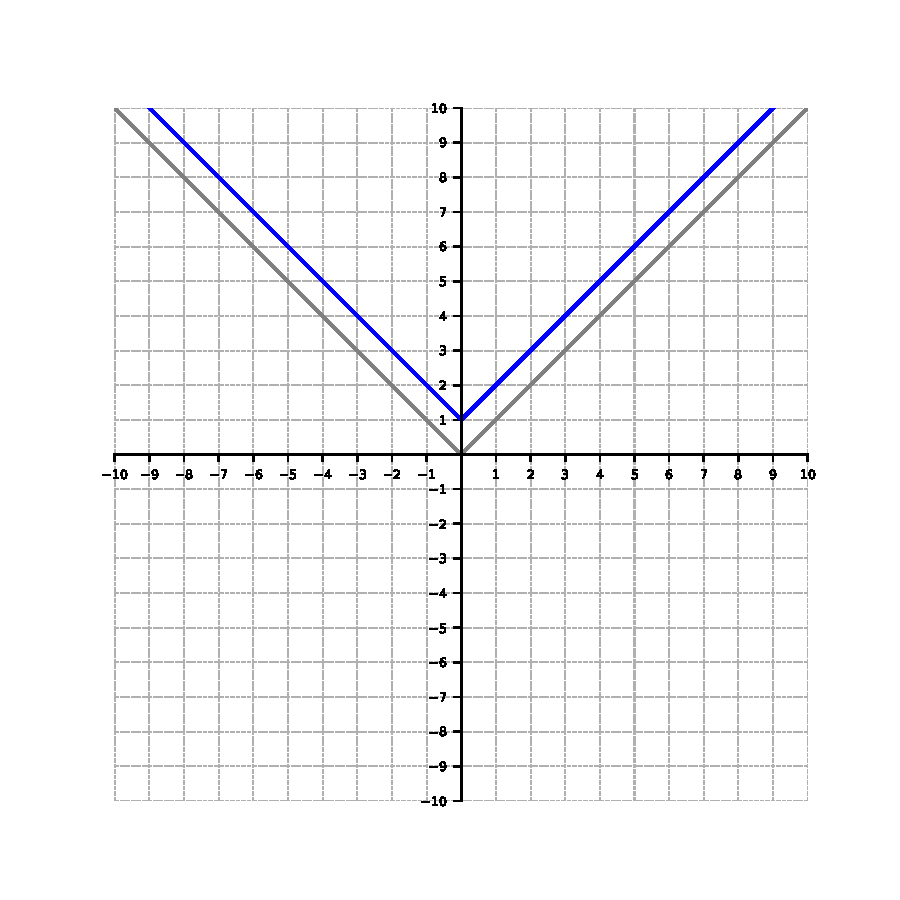
\includegraphics[width=0.5\textwidth]{figures/01_Relations_and_Functions/07_Transformations/exercise_19.pdf}
          \end{center}
    \item[64.]
          \[g(x) = 2f(-x -3) - 1 = 2 \sqrt[3]{-x - 3} - 1\]
\end{enumerate}